\documentclass{article}

\usepackage[utf8]{inputenc} %cp1252 pour Windows, utf8 pour Linux
\usepackage[T1]{fontenc}
\usepackage{lmodern}
\usepackage{graphicx}
\usepackage[french]{babel}
\usepackage{hyperref}

\title{La médecine de guerre dans ArmA III}
\author{Heartbroken}
\date{\today}

\newcommand{\arma}{\emph{ArmA III}}
\newcommand{\version}{\texttt{Version 1.0}}
\newcommand{\medsys}{\emph{ACE3} Basic Medical System}

\begin{document}
	
	\maketitle
	
	\begin{figure}[h]
		\centerline{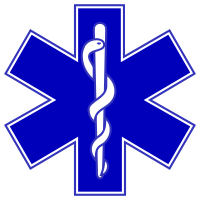
\includegraphics{Star_of_life2}}
	\end{figure}
	
	\begin{abstract}
		
		Ce court tutoriel a pour but d'initier à la pratique de la médecine de guerre dans \arma. Pour les utilisateurs déjà expérimentés ce document restera malgré tout particulièrement utile car il permettra de poser des standards pour les équipements, règles et réflexes à avoir. Enfin il est important de préciser qu'il n'est pas uniquement édité à l'attention des joueurs voulant jouer un rôle médical mais bien à tous les joueurs. Ainsi chaque partie contiendra dans la mesure du possible une section pour le fantassin de base. Cependant il est conseillé même au joueurs ne voulant pas jouer de rôle médical de lire les sections concernant ceux-ci afin de mieux comprendre et de pouvoir anticiper les actions des personnels médicaux.
		
	\end{abstract}
	
		\begin{center}
			
			\medsys
			
			\version
			
		\end{center}
	
	\newpage
	
	\part{Dégagement de responsabilités}
		\emph{L'auteur tient à faire noter que bien que ce tutoriel est basé sur de véritables notions de secourisme appliquées dans le monde réel ce document ne remplace pas les diverses formations civiles (\emph{PSC1, PSE1}\dots) et militaires de secours à personne. En effet une certaine liberté est prise sur divers aspects qui sont très simplifiés voire absents de par les limitations d'\arma\ et des mods employés. Ainsi l'auteur ne peut être tenu responsable de tout incident, accident, blessure ou décès causés par une méconnaissance des gestes qui sauvent et/ou d'une application de ce document et son contenu dans la vie réelle.}
		
	\part{Assomptions initiales}
		Comme indiqué en page de garde ce tutoriel est centré sur le système médical "\medsys\ ". Il est important de préciser que certains éléments de ce document pourrait justement devenir caduques face à l'Advanced Medical System qui comme son nom l'indique est plus avancé sur une majorité d'éléments. De plus l'auteur part du principe que le lecteur sait déjà utiliser les fonctions de base du \emph{ACE3}. Ainsi que ce soit le "Self-Interaction Menu" et plus simplement "l'Interaction Menu" on supposera déjà connu et acquis leur utilisation. Enfin ce document ne remplace pas une courte formation initiale sur le menu médical contextuel et/ou le "Medical Menu" dont l'emploi est lui aussi supposé connu du lecteur. Enfin il est admis que les lecteurs jouant les rôles médicaux ont déjà eu au préalable un formation spécifique à leurs postes, ce document étant plus un appui de formation, pas un remplacement.
	
	\part{Chaîne médicale militaire}
		\begin{figure}[h]
			\centerline{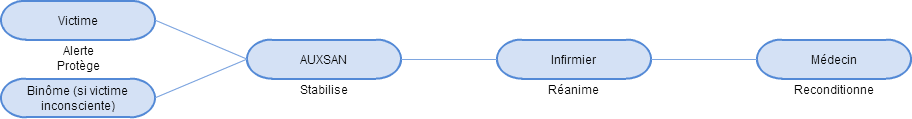
\includegraphics[scale=0.6]{FlowchartSecoursMilitaire}}
			\caption{\label{FlowchartSecoursMilitaire} Chaîne médicale militaire simplifiée}
		\end{figure}
		Dans \arma\ la chaîne des secours est relativement simplifiée. Malgré les ajouts de \emph{ACE3} le fait que de se limiter au \medsys\ bien que rendant un peu plus complet et proche de la réalité la chaîne des secours elle reste un peu plus simple. En particulier le rôle du médecin est ici uniquement sémantiquement différent de celui de l'infirmier. Cette partie va s'atteler à expliquer la prise en charge théorique d'une victime suite à un combat telle que représenté dans la figure \ref{FlowchartSecoursMilitaire}. Il est évident que cette chaîne est comme tout élément soumis aux opérations et ne sera probablement pas appliquée dans son intégralité par manque de temps, de personnels ou encore par les effets de tirs ennemis.\\
		
		Pour mieux expliquer la chaîne des secours mettons-nous en situation. Un personnel est blessé au cours des opérations, deux possibilités s'ouvrent alors. La première est que malgré ses blessures la victime est consciente. Alors elle donne l'alerte elle-même sur sa situation. Si la victime est rendue inconsciente par ses blessures alors ce sera à son binôme, ou à son découvreur le cas échéant, de donner l'alerte. L'alerte est l'étape la plus importante finalement car si elle est pas/mal faite alors les secours peuvent ne pas venir du tout. Enfin l'alerte donnée la victime assure son auto-protection et celle des secours qui vont arriver. Le cas échéant ce sera au binôme de protéger la victime et les secours tout en ne se mettant pas en danger inutilement.\\
		
		Le premier maillon de la chaîne médicale qui devrait arriver est donc l'AUXSAN de l'unité. Généralement il n'est jamais très loin du front et peut donc arriver très rapidement sur une victime ou la victime elle-même peut simplement aller le voir. De plus de par son équipement il peut bien plus facilement se défendre tout seul. Cependant de par la toute relative compétence médicale de l'AUXSAN et son manque d'équipement son but est purement et simplement de stabiliser une victime. Ainsi il va dans les limites de son matériel tenre de stopper ou au moins réduire les saignements de la victime. Par contre l'AUXSAN va aussi pouvoir faire un bilan bien plus complet de la victime à transmettre au besoin. Après que l'AUXSAN soit intervenu il reste au côté de la victime si celle-ci est encore inconsciente et attend l'intervention de l'infirmier de l'unité. \\
		
		Dans la plupart des cas où un AUXSAN est présent l'infirmier ne se déplacera pas pour des personnels conscients et stabilisés, il assistera la victime quand la situation le permettra mais ne risquera pas de se mettre en danger. En effet seul l'infirmier est habilité à administrer quelques solutions médicamenteuses (morphine, adrénaline/épinéphrine, atropine\dots) que ce soit. Cela permet d'éviter au maximum les overdoses puisque l'infirmier devrait normalement avoir noter, ou au moins se rappeler du nombre de sirettes administrées et quand. Ainsi le but de l'infirmier sera de terminer la stabilisation des patients que l'AUXSAN n'est pas dans la capacité de traiter, de s'occuper des douleurs perçues suite aux blessures mais surtout de réanimer les personnels inconscients. Enfin dans le cas de victimes nécessitant de la chirurgie (pas représenté dans le \medsys) ou alors suite à des manques de matériel l'infirmier peut décider avec l'accord du Chef de Groupe de procéder à une EVASAN de/des victimes les plus graves vers la base ou un poste médical avancé. C'est seulement de cette façon qu'une victime est amenée à rencontrer un médecin. En effet ceux-ci ne doivent jamais être proche du front (sauf ceux embarqués dans des MEDEVAC évidemment).\\
		
		
		%Paragraphe rôle médecin
		
	\part{Perception d'équipement}
		Avant de partir au feu il faut s'équiper. L'étape obligatoire de la perception de l'équipement est essentielle. La plupart des bons Game Masters vous auront déjà équipé plus ou moins correctement. Cependant il est toujours utile de vérifier votre équipement, de savoir pourquoi et à quoi il sert. C'est d'autant plus vrai dans la préparation au départ sur les missions improvisées pour lesquelles le Game Master n'aura probablement pas eu le temps de préparer un loadout médical. Cette partie va tenter de vous informer sur ce qui paraît pour l'auteur être le minimum requis en matière de matériel médical avant de partir en mission.
		
		\section{Pour le fantassin de base}
			Lorem ipsum dolor sit amet, consectetur adipiscing elit. Proin quis elit quam. Mauris non lorem ultricies, rhoncus nisl ut, blandit ante. Pellentesque tempus posuere tortor id consectetur. Nullam eu facilisis lectus. Proin vel leo sit amet sem malesuada hendrerit. Mauris id augue ornare, facilisis augue in, egestas sapien. Mauris vitae tincidunt leo. Nunc sapien turpis, sollicitudin id magna sed, interdum vehicula quam. Morbi nunc ligula, pharetra et ipsum vitae, ornare porta dui. Quisque sit amet nisi vitae nisl condimentum aliquet. Vivamus efficitur finibus purus fermentum eleifend. Vivamus ut magna et magna placerat efficitur suscipit id erat. Ut tellus ex, aliquam non neque id, porta consequat nisl.
			
		\section{Pour les personnels médicaux}
			En théorie chaque type de rôle médical ne devrait pas avoir exactement le même équipement car ils n'interviennent pas de la même façon sur les victimes. Cependant dans le \medsys\ il est vrai que la différence entre les rôles est principalement sémantique mais ici chaque rôle sera quand même séparé.
		
			\subsection{Médecins}
				Lorem ipsum dolor sit amet, consectetur adipiscing elit. Proin quis elit quam. Mauris non lorem ultricies, rhoncus nisl ut, blandit ante. Pellentesque tempus posuere tortor id consectetur. Nullam eu facilisis lectus. Proin vel leo sit amet sem malesuada hendrerit. Mauris id augue ornare, facilisis augue in, egestas sapien. Mauris vitae tincidunt leo. Nunc sapien turpis, sollicitudin id magna sed, interdum vehicula quam. Morbi nunc ligula, pharetra et ipsum vitae, ornare porta dui. Quisque sit amet nisi vitae nisl condimentum aliquet. Vivamus efficitur finibus purus fermentum eleifend. Vivamus ut magna et magna placerat efficitur suscipit id erat. Ut tellus ex, aliquam non neque id, porta consequat nisl.
				
			\subsection{Infirmiers}
				Lorem ipsum dolor sit amet, consectetur adipiscing elit. Proin quis elit quam. Mauris non lorem ultricies, rhoncus nisl ut, blandit ante. Pellentesque tempus posuere tortor id consectetur. Nullam eu facilisis lectus. Proin vel leo sit amet sem malesuada hendrerit. Mauris id augue ornare, facilisis augue in, egestas sapien. Mauris vitae tincidunt leo. Nunc sapien turpis, sollicitudin id magna sed, interdum vehicula quam. Morbi nunc ligula, pharetra et ipsum vitae, ornare porta dui. Quisque sit amet nisi vitae nisl condimentum aliquet. Vivamus efficitur finibus purus fermentum eleifend. Vivamus ut magna et magna placerat efficitur suscipit id erat. Ut tellus ex, aliquam non neque id, porta consequat nisl.
			
			\subsection{Auxilliaires Sanitaires}
				Lorem ipsum dolor sit amet, consectetur adipiscing elit. Proin quis elit quam. Mauris non lorem ultricies, rhoncus nisl ut, blandit ante. Pellentesque tempus posuere tortor id consectetur. Nullam eu facilisis lectus. Proin vel leo sit amet sem malesuada hendrerit. Mauris id augue ornare, facilisis augue in, egestas sapien. Mauris vitae tincidunt leo. Nunc sapien turpis, sollicitudin id magna sed, interdum vehicula quam. Morbi nunc ligula, pharetra et ipsum vitae, ornare porta dui. Quisque sit amet nisi vitae nisl condimentum aliquet. Vivamus efficitur finibus purus fermentum eleifend. Vivamus ut magna et magna placerat efficitur suscipit id erat. Ut tellus ex, aliquam non neque id, porta consequat nisl.
	
	\part{Actes réflexes}
		Lorem ipsum dolor sit amet, consectetur adipiscing elit. Proin quis elit quam. Mauris non lorem ultricies, rhoncus nisl ut, blandit ante. Pellentesque tempus posuere tortor id consectetur. Nullam eu facilisis lectus. Proin vel leo sit amet sem malesuada hendrerit. Mauris id augue ornare, facilisis augue in, egestas sapien. Mauris vitae tincidunt leo. Nunc sapien turpis, sollicitudin id magna sed, interdum vehicula quam. Morbi nunc ligula, pharetra et ipsum vitae, ornare porta dui. Quisque sit amet nisi vitae nisl condimentum aliquet. Vivamus efficitur finibus purus fermentum eleifend. Vivamus ut magna et magna placerat efficitur suscipit id erat. Ut tellus ex, aliquam non neque id, porta consequat nisl.
		
		\section{Pour le fantassin de base}
			Malgré tous vos efforts l'un des membres de votre unité vient d'être blessé. Deux possibilités s'ouvrent alors. La première et la plus heureuse est que la victime est encore consciente malgré ses blessures. La priorité est alors d'alerter de vive voix ou à la radio ses collègues de sa situation, de sa gravité (s'il a eu le temps de vérifier) et de sa position. Il est évidemment préférable d'avertir directement les personnels médicaux mais n'importe quel collègue fera l'affaire. Le blessé doit alors faire son possible pour se protéger et être en mesure de couvrir les personnels qui vont venir à son assistance. Si la gravité de la blessure le nécessite le blessé peut faire usage de ses bandages pour se stabiliser mais la prise de morphine est à proscrire. La deuxième est que la victime est tombée inconsciente suite à ses blessures. Dans ce cas-là c'est au binôme de celle-ci de passer l'alerte. Ceci fait il faut pouvoir mettre en sécurité la victime. Cela peut être fait en traînant celle-ci hors du feu, en la portant vers une zone plus sécurisée (plus long à mettre en œuvre mais déplacement plus rapide) ou simplement par l'usage de fumigènes ou d'une augmentation du feu. Par contre il est essentiel de noter que le binôme ne doit pas se mettre plus en danger que nécessaire en essayant de protéger la victime. La situation dictera ce qui est "se mettre trop en danger". Le binôme devra alors attendre et protéger les personnels médicaux qui arriveront. Si la situation le permet il peut faire, en attendant leur arrivée, un diagnostic de la victime voire la stabiliser si son état le nécessite (dans ce cas-là on ne donnera jamais de morphine à une victime inconsciente). Cependant cela ne devrait jamais résulter en une mise en danger de la victime, du binôme et des personnels de secours en transit.\\
			
			Si vous faîtes correctement votre travail et qu'aucun imprévu ne vienne l'empêcher, les premiers secours devraient arriver assez vite. Mais attention, leur arrivée ne veut pas dire que vous avez fini votre travail et que vous pouvez repartir gambader. En effet tout intervenant sur une victime est extrêmement vulnérable pendant qu'il administre les premiers soins. Il est donc essentiel de continuer de couvrir celui-ci. De plus l'intervention médicale sera d'autant plus courte que vous serez capable de transmettre certaines informations essentielles aux secouristes. Celles-ci sont les suivantes, si vous ne pouvez toutes les donner essayez quand même d'en fournir un maximum :
			\begin{itemize}
				\item dans le cas où vous êtes la victime et vous êtes désormais conscient, préciser que vous avez été inconscient
				\item préciser la cause des blessures (tirs ennemis, chute, surpression\dots)
				\item préciser la gravité générale des blessures
				\item préciser la localisation des blessures
				\item préciser les gestes de secours effectués
				\item (en supposant que vous avez passé outre les consignes de ne pas injecter soi-même de morphine) préciser la prise ou non de morphine, si oui combien et quand était la dernière prise
			\end{itemize}
			Cette passation d'information est bien plus facile à faire par la victime si elle est consciente car elle seule sera en mesure de donner toutes les informations aux personnels qualifiés. Cependant cela ne veut pas dire non plus que face à une victime inconsciente son binôme (ou découvreur dans le pire des cas) doit passer outre cette étape. Une fois tout ceci fait votre job en tant que fantassin est "fini" il ne vous reste plus qu'à protéger les personnels en train de techniquer la victime ou vous-même le cas échéant.
			
		\section{Pour les personnels médicaux}
			Lorem ipsum dolor sit amet, consectetur adipiscing elit. Proin quis elit quam. Mauris non lorem ultricies, rhoncus nisl ut, blandit ante. Pellentesque tempus posuere tortor id consectetur. Nullam eu facilisis lectus. Proin vel leo sit amet sem malesuada hendrerit. Mauris id augue ornare, facilisis augue in, egestas sapien. Mauris vitae tincidunt leo. Nunc sapien turpis, sollicitudin id magna sed, interdum vehicula quam. Morbi nunc ligula, pharetra et ipsum vitae, ornare porta dui. Quisque sit amet nisi vitae nisl condimentum aliquet. Vivamus efficitur finibus purus fermentum eleifend. Vivamus ut magna et magna placerat efficitur suscipit id erat. Ut tellus ex, aliquam non neque id, porta consequat nisl.
			
	\part{Incidents à nombreuses victimes, le Triage}
		Lorem ipsum dolor sit amet, consectetur adipiscing elit. Proin quis elit quam. Mauris non lorem ultricies, rhoncus nisl ut, blandit ante. Pellentesque tempus posuere tortor id consectetur. Nullam eu facilisis lectus. Proin vel leo sit amet sem malesuada hendrerit. Mauris id augue ornare, facilisis augue in, egestas sapien. Mauris vitae tincidunt leo. Nunc sapien turpis, sollicitudin id magna sed, interdum vehicula quam. Morbi nunc ligula, pharetra et ipsum vitae, ornare porta dui. Quisque sit amet nisi vitae nisl condimentum aliquet. Vivamus efficitur finibus purus fermentum eleifend. Vivamus ut magna et magna placerat efficitur suscipit id erat. Ut tellus ex, aliquam non neque id, porta consequat nisl.
		
		\section{Pour le fantassin de base}
			Lorem ipsum dolor sit amet, consectetur adipiscing elit. Proin quis elit quam. Mauris non lorem ultricies, rhoncus nisl ut, blandit ante. Pellentesque tempus posuere tortor id consectetur. Nullam eu facilisis lectus. Proin vel leo sit amet sem malesuada hendrerit. Mauris id augue ornare, facilisis augue in, egestas sapien. Mauris vitae tincidunt leo. Nunc sapien turpis, sollicitudin id magna sed, interdum vehicula quam. Morbi nunc ligula, pharetra et ipsum vitae, ornare porta dui. Quisque sit amet nisi vitae nisl condimentum aliquet. Vivamus efficitur finibus purus fermentum eleifend. Vivamus ut magna et magna placerat efficitur suscipit id erat. Ut tellus ex, aliquam non neque id, porta consequat nisl.
			
		\section{Pour les personnels médicaux}
			Lorem ipsum dolor sit amet, consectetur adipiscing elit. Proin quis elit quam. Mauris non lorem ultricies, rhoncus nisl ut, blandit ante. Pellentesque tempus posuere tortor id consectetur. Nullam eu facilisis lectus. Proin vel leo sit amet sem malesuada hendrerit. Mauris id augue ornare, facilisis augue in, egestas sapien. Mauris vitae tincidunt leo. Nunc sapien turpis, sollicitudin id magna sed, interdum vehicula quam. Morbi nunc ligula, pharetra et ipsum vitae, ornare porta dui. Quisque sit amet nisi vitae nisl condimentum aliquet. Vivamus efficitur finibus purus fermentum eleifend. Vivamus ut magna et magna placerat efficitur suscipit id erat. Ut tellus ex, aliquam non neque id, porta consequat nisl.			
	
	\newpage
	
	\tableofcontents
	
\end{document}